%!TEX root = ../thesis.tex  % Comment this line for standalone compilation
%*******************************************************************************
%*********************************** First Chapter Appendix *****************************
%*******************************************************************************

\chapter{Non-Uniform Diffusion Models}  %Title of the First Chapter

\section{Proofs}
\label{ch2:appendix:proofs}
\subsection{Equality of minimizers for CDE}
\label{ch2:appendix:minimizers}
\begin{lemma}
    \label{ch2:Vincent}
    For a fixed $y \in \mathbb{R}^d$ and $t \in \mathbb{R}$ we have
    \begin{align*}
        &\mathbb{E}_{\subalign{&x_0 \sim p(x_0 | y) \\ &x_t \sim p(x_t | x_0, y)}} 
            [\lambda(t) \norm{\nabla_{x_t} \ln{p(x_t | x_0, y)} - s_\theta(x_t, y, t)}_2^2]\\
        =& \mathbb{E}_{\subalign{&x_t \sim p(x_t |  y)}} 
            [\lambda(t) \norm{\nabla_{x_t} \ln{p(x_t | y)} - s_\theta(x_t, y, t)}_2^2]
    \end{align*}
\begin{proof}
    Since $y$ and $t$ are fixed, we may define $\psi(x_t) := s_\theta(x_t, y, t)$, $q(x_0) := p(x_0 | y)$ and $q(x_t | x_0) = p(x_t | x_0, y)$.
    Therefore, by the Tower Law, the statement of the lemma is equivalent to
    \begin{align*}
        &\mathbb{E}_{\subalign{&x_0, x_t \sim q(x_0, x_t)}} 
        [\norm{\nabla_{x_t} \ln{q(x_t | x_0)} - \psi(x_t)}_2^2]\\
    =& \mathbb{E}_{\subalign{&x_t \sim q(x_t)}} 
        [\norm{\nabla_{x_t} \ln{q(x_t)} - \psi(x_t)}_2^2]
    \end{align*}
    Which follows directly from \cite[Eq. 11]{vincent2011connection}.
\end{proof}
    
\end{lemma}
\begin{customthm}{1}
    The minimiser of
    \begin{gather*}
    \begin{aligned}
            &\frac{1}{2} \mathbb{E}_{\subalign{&t \sim U(0,T)\\ &x_0, y \sim p(x_0, y) \\ &x_t \sim p(x_t | x_0)}} 
            [\lambda(t) \norm{\nabla_{x_t} \ln{p(x_t | x_0)} - s_\theta(x_t, y, t)}_2^2]
    \end{aligned}
    \end{gather*}    
    in $\theta$ is the same as the minimiser of 
    \begin{gather*}
         \frac{1}{2} \mathbb{E}_{\subalign{&t \sim U(0,T)\\ &x_t, y \sim p(x_t, y)}} 
        [\lambda(t) \norm{\nabla_{x_t} \ln{p(x_t | y)} - s_\theta(x_t, y,t)}_2^2].
    \end{gather*}
\end{customthm}
\begin{proof}
    First, notice that $x_t$ is conditionally independent of $y$ given $x_0$. Therefore, by applying the Tower Law we obtain
    \begin{align*}
        &\mathbb{E}_{\subalign{&t \sim U(0,T)\\ &x_0, y \sim p(x_0, y) \\ &x_t \sim p(x_t | x_0)}} 
            [\lambda(t) \norm{\nabla_{x_t} \ln{p(x_t | x_0)} - s_\theta(x_t, y, t)}_2^2] \\
            \overset{(1)}{=}& \mathbb{E}_{\subalign{&t \sim U(0,T)\\ &y \sim p(y)\\&x_0 \sim p(x_0 | y) \\ &x_t \sim p(x_t | x_0)}} 
            [\lambda(t) \norm{\nabla_{x_t} \ln{p(x_t | x_0)} - s_\theta(x_t, y, t)}_2^2] \\
            \overset{(2)}{=}& \mathbb{E}_{\subalign{&t \sim U(0,T)\\ &y \sim p(y)\\&x_0 \sim p(x_0 | y) \\ &x_t \sim p(x_t | x_0, y)}} 
            [\lambda(t) \norm{\nabla_{x_t} \ln{p(x_t | x_0, y)} - s_\theta(x_t, y, t)}_2^2] \\ 
            =& \mathbb{E}_{\subalign{&t \sim U(0,T)\\ &y \sim p(y)}} 
            [f(t,y)] =: (*)
    \end{align*}
    where 
    \begin{align*}
        f&(t,y) := \\
        &\mathbb{E}_{\subalign{&x_0 \sim p(x_0 | y) \\ &x_t \sim p(x_t | x_0, y)}} [
        \lambda(t) \norm{\nabla_{x_t} \ln{p(x_t | x_0, y)} - s_\theta(x_t, y, t)}_2^2
    ].
    \end{align*}
    Now fix $y$ and $t$. By Lemma \ref{ch2:Vincent}, it follows that
    \begin{align*}
        &f(t,y) \\
        =&\mathbb{E}_{\subalign{&x_0 \sim p(x_0 | y) \\ &x_t \sim p(x_t | x_0, y)}} 
            [\lambda(t) \norm{\nabla_{x_t} \ln{p(x_t | x_0, y)} - s_\theta(x_t, y, t)}_2^2]\\
        \overset{(3)}{=}& \mathbb{E}_{\subalign{&x_t \sim p(x_t |  y)}} 
            [\lambda(t) \norm{\nabla_{x_t} \ln{p(x_t | y)} - s_\theta(x_t, y, t)}_2^2]\\
    \end{align*}
    Since $t$ and $y$ were arbitrary, this is true for all $t$ and $y$. Therefore, substituting back into $(*)$ we get that
    \begin{align*}
        (*) &= \mathbb{E}_{\subalign{&t \sim U(0,T)\\ &y \sim p(y)\\&x_t \sim p(x_t | y)}} 
            [\lambda(t) \norm{\nabla_{x_t} \ln{p(x_t | y)} - s_\theta(x_t, y, t)}_2^2]\\
        &\overset{(1)}{=} \mathbb{E}_{\subalign{&t \sim U(0,T)\\ &x_t, y \sim p(x_t, y)}} 
        [\lambda(t) \norm{\nabla_{x_t} \ln{p(x_t | y)} - s_\theta(x_t, y,t)}_2^2].
    \end{align*}
(1) Tower Law, (2) Conditional independence of $x_t$ and $y$ given $x_0$, (3) \text{Lemma} \ref{ch2:Vincent}.
\end{proof}

\subsection{Consistency of CDE}
\label{ch2:appendix:consistency}
In order to prove the consistency, in this subsection we make the following assumptions:
\begin{assumption}
    \label{ch2:assum:compact_1}
    The space of parameters $\Theta$ and the data space $\mathcal{X}$ are compact.
\end{assumption}
\begin{assumption}
    \label{ch2:assum:unique}
    There exists a unique $\theta^\ast \in \Theta$ such that $s_{\theta^\ast}(x,y,t) = \nabla_{x_t}\ln p (x,y,t)$.
\end{assumption}

First we state some technical, but well-known lemmas, which will be useful in proving our consistency result.

\begin{lemma}[Uniform law of large numbers] \cite[Lemma 2.4]{whitney1994estimation} \\
    \label{ch2:lemma:ULLN}
    Let $z_i$ be i.i.d from a distribution $q(z)$ and suppose that:
    \begin{itemize}
        \item $\Theta$ is compact.
        \item $f(z,\theta)$ is continuous for all $\theta \in \Theta$ and almost all $z$.
        \item $f(\cdot, \theta)$ is a measurable function of $z$ for each $\theta$.
        \item There exists $d: \mathcal{Z} \xrightarrow{} \mathbb{R}$ such that $\mathbb{E}[d(z)]<\infty$ and $\norm{f(z,\theta)} \leq d(z)$ for each $\theta$.
    \end{itemize}
    Then $\mathbb{E}_{z}[f(z,\theta)]$ is continuous in $\theta$, and $\frac{1}{n}\sum_{i=1}^n f(z_i, \theta)$ converges to $\mathbb{E}_{z}[f(z,\theta)]$ uniformly in probability, i.e.:
    \begin{gather*}
        \sup_\theta \norm{\frac{1}{n}\sum_{i=1}^n f(z_i, \theta) - \mathbb{E}_{z}[f(z,\theta)]} \overset{P}{\to} 0
    \end{gather*}

\end{lemma}

\begin{lemma}[Consistency of extremum estimators] \cite[Theorem 2.1]{whitney1994estimation} \\
    \label{ch2:lemma:consistency}
    Let $\Theta$ be compact and consider a family of functions $\mathcal{L}^{(n)}: \Theta \to \mathbb{R}$. Moreover, suppose there exists a function $\mathcal{L}: \Theta \to \mathbb{R}$ such that
    \begin{itemize}
        \item $\mathcal{L}(\theta)$ is uniquely minimised at $\theta^\ast$.
        \item $\mathcal{L}(\theta)$ is continuous.
        \item $\mathcal{L}^{(n)}(\theta)$ converges uniformly in probability to $\mathcal{L}(\theta)$.
    \end{itemize}
    Then $$\theta^\ast_n := \underset{\theta \in \Theta}{\arg\min} \, \mathcal{L}^{(n)}(\theta).$$
\end{lemma}


\begin{customcoll}{1}
    Let $\theta_n^\ast$ be a minimiser of a $n$-sample Monte Carlo approximation of \begin{gather*}
        \begin{aligned}
                \frac{1}{2} \mathbb{E}_{\subalign{&t \sim U(0,T)\\ &x_0, y \sim p(x_0, y) \\ &x_t \sim p(x_t | x_0)}} 
                [\lambda(t) \norm{\nabla_{x_t} \ln{p(x_t | x_0)} - s_\theta(x_t, y, t)}_2^2].
        \end{aligned}
        \end{gather*} 
        Then under assumptions \ref{ch2:assum:compact_1} and \ref{ch2:assum:unique}, the conditional denoising estimator $s_{\theta_n^\ast}(x,y,t)$ is a consistent estimator of the conditional score $\nabla_{x_t} \ln p(x_t | y)$, i.e.
    \begin{gather*}
        s_{\theta_n^\ast}(x,y,t) \overset{P}{\to} \nabla_{x_t} \ln p(x_t | y),
    \end{gather*}
    as the number of Monte Carlo samples $n$ approaches infinity.
\end{customcoll}

\begin{proof}
    By conditional independence and the Tower Law, we get
    \begin{align*}
         &\mathbb{E}_{\subalign{&t \sim U(0,T)\\ &x_0, y \sim p(x_0, y) \\ &x_t \sim p(x_t | x_0)}} 
                [\lambda(t) \norm{\nabla_{x_t} \ln{p(x_t | x_0)} - s_\theta(x_t, y, t)}_2^2] \\
        =& \mathbb{E}_{\subalign{&t \sim U(0,T)\\ &x_0, y \sim p(x_0, y) \\ &x_t \sim p(x_t | x_0, y)}} 
            [\lambda(t) \norm{\nabla_{x_t} \ln{p(x_t | x_0)} - s_\theta(x_t, y, t)}_2^2] \\
        =& \mathbb{E}_{\subalign{&t \sim U(0,T)\\ &x_0,, x_t, y \sim p(x_0, x_t ,y)}} 
            [\lambda(t) \norm{\nabla_{x_t} \ln{p(x_t | x_0)} - s_\theta(x_t, y, t)}_2^2].
    \end{align*}
    Let $z=(t,x_0,x_t,y)$ and denote by $q(z):=p(t,x_0,x_t,y)$ the joint distribution. Moreover, define $f(z,\theta) := \lambda(t) \norm{\nabla_{x_t} \ln{p(x_t | x_0)} - s_\theta(x_t, y, t)}_2^2$. Since $t \sim U(0,T)$ is independent of $(x_0, x_t ,y) \sim p(x_0, x_t ,y)$, the above is equal to 
    \begin{align*}
        \mathbb{E}_{z \sim q(z)} 
            [f(z,\theta)]
    \end{align*}
    Therefore by Lemma \ref{ch2:lemma:ULLN}, the Monte Carlo approximation of \ref{ch2:CDN}: $\mathcal{L}^{(n)}(\theta)=\frac{1}{n}\sum_{i=1}^n f(z_i, \theta)$ converges uniformly in probability to $\mathcal{L}(\theta) = \mathbb{E}_{z \sim q(z)} 
    [f(z,\theta)]$. Let $\theta^\ast$ be the minimiser of $\mathcal{L}(\theta)$, by Lemma \ref{ch2:lemma:consistency} we get that $\theta^\ast_n \overset{P}{\to} \theta^\ast$ . Finally by Theorem \ref{ch2:thm:CDE_consistency}, $\theta^\ast$ is also a minimiser of the Fisher divergence between $s_{\theta^\ast}(x_t,y,t)$ and $\nabla_{x_t} \ln p(x_t | y)$ and by Assumption \ref{ch2:assum:unique} this implies that $s_{\theta^\ast}(x_t,y,t) = \nabla_{x_t} \ln p(x_t | y)$. Hence $s_{\theta_n^\ast}(x,y,t) \overset{P}{\to} \nabla_{x_t} \ln p(x_t | y)$.
\end{proof}

\subsection{Likelihood weighting for multi-speed and multi-sde models}
\label{ch2:appendix:weighting}
In this section we derive the likelihood weighting for multi-sde models (Theorem \ref{ch2:thm:weightning}). First using the framework in \cite[Appendix A]{song2021sde} we present the Anderson's theorem for multi-dimensional SDEs with non-homogeneous covariance matrix (without assuming $\Sigma(t) \not = \sigma(t) I$) and generalise the main result of \cite{song2021maximum} to this setting. Then, we cast the problem of multi-speed and  multi-sde diffusion as a special case of multi-dimensional diffusion with a particular covariance matrix $\Sigma(t)$ and thus obtain the likelihood weighting for multi-sde models (Theorem \ref{ch2:thm:weightning}).

Consider an Ito's SDE
\begin{align*}
    dx = \mu(x, t)dt + \Sigma(t)dw
\end{align*}
where $\mu: \mathbb{R}^{n_x} \times [0,T] \xrightarrow{} \mathbb{R}^{n_x}$ and $\Sigma: [0,T] \xrightarrow{} \mathbb{R}^{n_x \times n_x}$ is a time-dependent positive-definite matrix. By multi-dimensional Anderson's Theorem \cite{anderson1982reverse_time_sde} the corresponding reverse time SDE is given by 
\begin{align}
    \label{ch2:eq:true_rtsde}
    dx &= \tilde{\mu}(x, t)dt + \Sigma(t)dw \\
    \text{where } \tilde{\mu}(x,t) &:= \mu(x,t) -  \Sigma(t)^2 \nabla_x \ln p_{X_t}(x). \nonumber
\end{align}

If we train a score-based diffusion model to approximate $\nabla_x \ln p_{X_t}(x)$ with a neural network $s_\theta(x,t)$ we will obtain the following approximate reverse-time sde
\begin{align}
    \label{ch2:eq:approx_rtsde}
    dx &= \tilde{\mu}_\theta(x, t)dt + \Sigma(t)dw \\
    \text{where } \tilde{\mu}_\theta(x,t) &:= \mu(x,t) -  \Sigma(t)^2 s_\theta(x,t) \nonumber
\end{align} 


Now we generalise \cite[Theorem 1]{song2021maximum} to multi-dimensional setting.
\begin{theorem} 
    Let $p(x_t)$ and $p_\theta(x_t)$ denote marginal distributions of \ref{ch2:eq:true_rtsde} and \ref{ch2:eq:approx_rtsde} respectively. Then under regularity assumptions of \cite[Theorem 1]{song2021maximum} we have that 
    \label{ch2:thm:multi-dim}
    \begin{equation}
        KL(p(x_0) | p_\theta(x_0)) \leq KL(p(x_T) | \pi(x_T)) + \frac{1}{2} \mathbb{E}_{\subalign{&t \sim U(0,T)\\ &x_t \sim p(x_t)}} [v^T \Sigma(t)^2 v],
    \end{equation}
    where $v=\nabla_{x_t} \ln{p(x_t)} - s_\theta(x_t,t)$. 
\end{theorem}

    
\begin{proof}   
    We proceed in close analogy to the proof of \cite[Theorem 1]{song2021maximum} but we use a more general diffusion matrix $\Sigma(t)$. 
    Let $P$ be the law of the true reverse-time sde and let $P_\theta$ be the law of the approximate reverse-time sde. 
    Then by  \cite[Theorem 2.4]{leonard2013properties} (generalised chain rule for KL divergence) we have
    \begin{equation}
        KL(P | P_\theta) = KL(p(x_0) | p_\theta(x_0)) + \mathbb{E}_{z \sim p(x_0)}[KL(P(\cdot | x_0=z) |P_\theta(\cdot | x_0=z))].
    \end{equation}
    
    Since $\mathbb{E}_{z \sim p(x_0)}[KL(P(\cdot | x_0=z) |P_\theta(\cdot | x_0=z))] \geq 0$, this implies 
    \begin{align*}
       KL(p(x_0) | p_\theta(x_0)) \leq KL(P | P_\theta) 
    \end{align*}
    Using the fact that $p_\theta(x_T) = \pi$ and applying \cite[Theorem 2.4]{leonard2013properties} again, we obtain
    \begin{equation}
        KL(P | P_\theta) = KL(p(x_T) |\pi) + \mathbb{E}_{z \sim p(x_T)}[KL(P(\cdot | x_T=z) |P_\theta(\cdot | x_T=z))].
    \end{equation}    
    Let $P^z := P(\cdot | x_T=z)$ and $P_\theta^z := P_\theta(\cdot | x_T=z)$
    \begin{equation}
        \mathbb{E}_{z \sim p(x_T)}[KL(P(\cdot | x_T=z) |P_\theta(\cdot | x_T=z))] = - \mathbb{E}_{z \sim p(x_T)} \left[ \mathbb{E}_{P^z} \left[ \ln \frac{d P^z_\theta}{d P^z} \right] \right].
    \end{equation}    
    Using Girsanov Theorem \cite[Theorem 8.6.5]{oksendal2003sde} and the fact that $\Sigma(t)$ is symmetric and invertible 
    \begin{equation}
        \mathbb{E}_{z \sim p(x_T)} \left[ \mathbb{E}_{P^z} \left[ \int_0^T \Sigma(t) v(x_t,t) dw_t + \frac{1}{2} \int_0^T v(x_t,t)^T \Sigma(t)^2 v(x_t,t) dt \right] \right].
    \end{equation}    
    where $v(x_t,t)=\nabla_{x_t} \ln{p(x_t)} - s_\theta(x_t,t)$. Since $\int_0^T  \Sigma(t) v(x_t,t) dw_t $ is a martingale (Ito's integral wrt Brownian motion) 
    \begin{align*}
        &=  \frac{1}{2} \mathbb{E}_{z \sim p(x_T)}  \bigg[ 
            \mathbb{E}_{P^z} \bigg[
                     \int_0^T v(x_t,t)^T \Sigma(t)^2 v(x_t,t) dt 
            \bigg]
        \bigg] \\
        &= \frac{1}{2} \int_0^T \mathbb{E}_{x \sim p(x_t)}[ v(x_t,t)^T \Sigma(t)^2 v(x_t,t)] \\
        &= \frac{1}{2} \mathbb{E}_{\subalign{&t \sim U(0,T)\\ &x_t \sim p(x_t)}} 
        [
            v(x_t,t)^T \Sigma(t)^2 v(x_t,t)
        ].
    \end{align*}
\end{proof}

\subsubsection{Multi-sde and multi-speed diffusion}
Now we consider again the multi-speed and the more general multi-sde diffusion frameworks from sections \ref{ch2:sec:multi-scale_diffusion} and \ref{ch2:sec:conditional_generation}. Suppose that we have two tensors $x$ and $y$ which diffuse according to different SDEs
\begin{gather*}
    dx = \mu^x(x,t)dt+\sigma^x(t)dw  \\
    dy = \mu^y(y,t)dt+\sigma^y(t)dw  
\end{gather*}
We may cast this system of two SDEs, as a single SDE
\begin{gather*}
    dz = \mu^z(z,t)dt+ \Sigma_z(t)dw 
\end{gather*}
where $z = (x,y)$, $\mu^z(z,t) = (\mu^x(x,t), \mu^y(x,t))$ and 
\begin{gather*}
    \Sigma_z(t) =  
    \begin{cases} 
        \sigma^x(t), \text{ if } i=j, \ i \leq n_x \\ 
        \sigma^y(t), \text{ if } i=j, \ n_x < i \leq n_y  \\
        0, \text{ otherwise}
    \end{cases}
    .            
\end{gather*}
If we train a score-based diffusion model for $z_t = (x_t, y_t)$, then by Theorem \ref{ch2:thm:multi-dim}
\begin{align*}
    KL(p(z_0) | p_\theta(z_0)) \leq C_1 + \frac{1}{2} \mathbb{E}_{\subalign{&t \sim U(0,T)\\ &z_t \sim p(z_t)}} 
    [
        v^T \Sigma_z(t)^2 v
    ],
\end{align*}
where $C_1 := KL(p(x_T) | \pi(x_T)) $ does not depend on $\theta$.
Because $\Lambda_{MLE}$ (from Theorem \ref{ch2:thm:weightning}) is equal to $\Sigma_z(t)^2$, we may rewrite the above as 
\begin{align*}
    KL(p(z_0) | p_\theta(z_0)) \leq C_1 + \frac{1}{2} \mathbb{E}_{\subalign{&t \sim U(0,T)\\ &z_t \sim p(z_t)}} 
    [
        v^T \Lambda_{MLE}(t)^2 v
    ],
\end{align*}
and since by denoising score matching \cite{vincent2011connection} 
\begin{equation}
    \mathbb{E}_{\subalign{&t \sim U(0,T)\\ &z_t \sim p(z_t)}} \left[ v^T \Lambda_{MLE}(t) v \right] = \mathbb{E}_{\subalign{&t \sim U(0,T)\\ &z_0 \sim p_0(z_0) \\ &z_t \sim p(z_t | z_0)}} \left[ v^T \Lambda_{MLE}(t) v \right] + C_2.
\end{equation}

where $C_2$ is another term constant in $\theta$.
We conclude that 
\begin{align*}
    KL(p(z_0) | p_\theta(z_0)) \leq \frac{1}{2} \mathbb{E}_{\subalign{&t \sim U(0,T)\\ &z_0 \sim p_0(z_0) \\ &z_t \sim p(z_t | z_0)}} 
    [
        v^T \Lambda_{MLE}(t) v
    ] + C_3
\end{align*}
where $C_3 := C_1 + C_2$.
Now recall that the term on the RHS is exactly the training objective of a multi-sde score-based diffusion model with likelihood weighting
\begin{gather*}
    \begin{aligned}
        \mathcal{L}(\theta) := \frac{1}{2} \mathbb{E}_{\subalign{&t \sim U(0,T)\\ &z_0 \sim p_0(z_0) \\ &z_t \sim p(z_t | z_0)}} 
        [
            v^T \Lambda_{MLE}(t) v
        ].
    \end{aligned}
\end{gather*}
Therefore
\begin{align*}
    KL(p(z_0) | p_\theta(z_0)) \leq \mathcal{L}(\theta)  + C_3.
\end{align*}
Finally, since $KL(p(z_0) | p_\theta(z_0))  = \mathbb{E}_{(x,y) \sim p(x,y)}[\ln p(x,y)]  - \mathbb{E}_{(x,y) \sim p(x,y)}[\ln p_\theta(x,y)]$, we have 
\begin{gather*}
    -\mathbb{E}_{(x,y) \sim p(x,y)}[\ln p_\theta(x,y)] \leq \mathcal{L}(\theta) + C
\end{gather*}
where $C := C_3 - \mathbb{E}_{(x,y) \sim p(x,y)}[\ln p(x,y)] $ is independent of $\theta$. Thus the Theorem \ref{ch2:thm:weightning} is established.

\subsection{Mean square approximation error}
\label{ch2:appendix:mse}

\begin{assumption}
    \label{ch2:assum:_c2}
    $p(x,y) \in C^2(\mathcal{X})$\
\end{assumption}
\begin{assumption}
    \label{ch2:assum:_lower_bound}
    $p(x,y) > 0$ for all $x,y$.
\end{assumption}
\begin{assumption}
    \label{ch2:assum:_compact_2}
    The data space $\mathcal{X}$ is compact.
\end{assumption}

\begin{lemma}
    \label{ch2:lemma:_blurring}
    Under assumptions \ref{ch2:assum:_c2} and \ref{ch2:assum:_compact_2} we have
    \begin{gather*}
        p_{Y_t | X_t}(y_t | x_t)  = (p_{Y | X_t}(\cdot | x_t) \ast \varphi_\sigma)(y_t) \\
        \partial_{x_t} p_{Y_t | X_t}(y_t | x_t) = (\partial_{x_t} p_{Y| X_t}(\cdot | x_t) \ast \varphi_\sigma)(y_t)
    \end{gather*}
\end{lemma}
\begin{proof}
    For this proof, we drop our convention of denoting the probability distribution of a random variable via the name of its density’s argument.
    \begin{align*}
        p_{Y_t | X_t}(y_t | x_t)  &= \int p_{Y, Y_t| X_t}(y, y_t | x_t) dy 
        \\ &= \int p_{Y | X_t}(y | x_t) p_{Y_t |Y, X_t}(y_t | y, x_t) dt
        \\ &= \int p_{Y | X_t}(y | x_t) p_{Y_t |Y}(y_t | y) dy
    \end{align*}
    Since $Y_t |Y$ has normal distribution with mean $y$ and variance $\sigma^y(t)^2$:
    \begin{align*}
        &= \int p_{Y | X_t}(y | x_t) \varphi_\sigma(y_t - y)  dy 
        \\ &= (p_{Y | X_t}(\cdot | x_t) \ast \varphi_\sigma)(y_t)
    \end{align*}
    where $\varphi_\sigma$ is a Gaussian kernel with variance $\sigma^y(t)^2$.
    Moreover, under the assumptions of the lemma we can exchange the differentiaion and integration. Therefore
    \begin{align*}
        \partial_{x_t} p_{Y_t | X_t}(y_t | x_t) &= \partial_{x_t} \int p_{Y | X_t}(y | x_t) \varphi_\sigma(y_t - y) dy   
        \\ &=  \int \partial_{x_t} p_{Y | X_t}(y | x_t) \varphi_\sigma(y_t - y) dy  
        \\ &= (\partial_{x_t} p_{Y | X_t}(\cdot | x_t) \ast \varphi_\sigma)(y_t)
    \end{align*}
\end{proof}

\begin{lemma}
    \label{ch2:lemma:_sup_norm}
    Let $f$ be a $C^1$-function on a compact domain $\mathcal{X}$ and let $\varphi_\sigma$ be a Gaussian kernel with variance $\sigma^2$. Then there exists a function $E: \mathbb{R} \xrightarrow{} \mathbb{R}$, which is monotonically decreasing to zero, such that
    \begin{gather*}
        \norm{(f \ast \varphi_\sigma) - f}_{\infty} \leq E(1/\sigma).
    \end{gather*}
\end{lemma}

\begin{proof}
    \begin{align*}
        & \phantom{=}|(f \ast \varphi_\sigma)(y) -f(y)| 
        \\&= \bigg| \int f(z)  \varphi_\sigma(z-y) dz - \int f(y) \varphi_\sigma(z-y) dz \bigg|
        \\&\leq  \int |f(z) -f(y)| \varphi_\sigma(z-y) dz
    \end{align*}
    Since $f$ is  a $C^1$ function on a compact domain, it is Lipschitz and bounded (in absolute value) by some constant $M$. 
    Fix $\epsilon > 0$, and let $L$ denote the Lipschitz constant of $f$.
    We have that $|f(z) -f(y)| < \epsilon$ whenever $\norm{z-y} < \epsilon / L$.
    Let $B_y( \epsilon / L ) := \{z \in \mathcal{X} : \norm{z-y} < \epsilon / L \}$ be a ball of radius $\epsilon / L$ around $y$.
    Then
    \begin{align*}
        &\phantom{=}\int |f(z) -f(y)| \varphi_\sigma(z-y) dz 
        \\ &\! \begin{aligned}
            = \int_{B_y( \epsilon / L )}& |f(z) -f(y)| \varphi_\sigma(z-y) dz 
            \\ &+ \int_{\mathcal{X} \setminus B_y( \epsilon / L )} |f(z) -f(y)| \varphi_\sigma(z-y) dz
        \end{aligned}
        \\ &\leq \epsilon +  \int_{\mathcal{X} \setminus B_y( \epsilon / L )}  2M \varphi_\sigma(z-y) dz
       \\ &= \epsilon +  2M P \left( |Z_\sigma| > \frac{\epsilon}{L} \right)
    \end{align*}
    where $Z_\sigma$ is a normally-distributed random variable with mean zero and variance $\sigma^2$.
    By the Chernoff bound, we have
    \begin{align*}
        \leq  \epsilon +  4M \exp \left( -\frac{\epsilon^2}{2L^2 \sigma^2}\right).
    \end{align*}
    
    \noindent Define $E_\epsilon(1/\sigma) :=   \epsilon +  4M \exp \left( -\frac{\epsilon^2}{2L^2 \sigma^2}\right)$. Observe that $E_\epsilon: \mathbb{R}_+ \xrightarrow{} \mathbb{R}$ is monotonically decreasing to $\epsilon$.
    Moreover 
    $$ \norm{(f \ast \varphi_\sigma) - f}_{\infty} \leq E_{\epsilon}(1/\sigma). $$
    Now let $A := [0,1]$ and define 
    $$E(1/\sigma) := \min_{\epsilon \in A} E_\epsilon(1/\sigma).$$
    Notice that the above minimum is achieved, since $A$ is compact and for a fixed $\sigma$, the function $\epsilon \mapsto E_{\epsilon}(1/\sigma)$ is continuous.

    We will prove that $E$ is a monotonically decreasing to zero and upper-bounds $\norm{(f \ast \varphi_\sigma) - f}_{\infty}$.
    Firstly, it is clear that $E(x) \to 0$ as $x \to \infty$, since for all $\epsilon \in A$ we have $\lim_{x \to \infty} E(x) \leq \lim_{x \to \infty} E_{\epsilon}(x)=\epsilon$ . 
    Secondly, suppose $a < b$, and let $\epsilon_a$ be such that $E(a) = E_{\epsilon_a}(a)$. Then
    $$E(b) = \inf_{\epsilon \in A} E_{\epsilon}(b) \leq E_{\epsilon_a}(b) < E_{\epsilon_a}(a) = E(a).$$
    Therefore $E$ is monotonically decreasing.
    Finally since for all $\epsilon > 0$
    $$ \norm{(f \ast \varphi_\sigma) - f}_{\infty} \leq E_{\epsilon}(1/\sigma). $$
    Taking minimum over $\epsilon \in A$ on both sides we obtain 
    $$ \norm{(f \ast \varphi_\sigma) - f}_{\infty} \leq E(1/\sigma). $$
\end{proof}


\begin{lemma}
    \label{ch2:lemma:_Lpz}
    Let $f$ be a $C^1$ function on a compact domain and let $Z$ be a random variable with mean $\mu$ and variance $\sigma^2$.
    Then
    \begin{gather*}
        \mathbb{E}_Z[(f(\mu) - f(Z))^2] \leq L^2 \sigma^2
    \end{gather*}
    where $L$ denotes the Lipschitz constant of $f$.
\end{lemma}
\begin{proof}
Since  $f$ is a $C^1$ function on a compact domain it is Lipschitz with some Lipschitz constant $L$. Therefore
\begin{align*}
    \mathbb{E}_Z[(f(\mu) - f(Z))^2] 
    \leq L^2\mathbb{E}_Z[(\mu - Z)^2]
    \leq L^2 \sigma^2
\end{align*}    
\end{proof}

\begin{customthm}{3}
    Fix $t$, $x_t$ and $y$. Then under Assumptions \ref{ch2:assum:_c2}, \ref{ch2:assum:_lower_bound} and \ref{ch2:assum:_compact_2}, there exists a function $E: \mathbb{R} \xrightarrow{} \mathbb{R}$ which is monotonically decreasing to zero, such that
    \[
\mathbb{E}_{y_t \sim p(y_t|y)}\left[\norm{ \nabla_{x_t} \ln p(x_t|y_t) - \nabla_{x_t} \ln p(x_t|y)}_2^2 \right] \leq E\left( \frac{1}{\sigma^y(t)} \right).
\]
\end{customthm}
\begin{proof}
    For this proof, we drop our convention of denoting the probability distribution of a random variable via the name of its density’s argument.
   \[
\norm{ \nabla_{x_t} \ln p_{X_t | Y_t}(x_t|y_t) - \nabla_{x_t} \ln p_{X_t | Y}(x_t|y)}_2^2
= \sum_{i=1}^{n_x} \left( \partial^i_{x_t} \ln p_{X_t | Y_t}(x_t|y_t) - \partial^i_{x_t} \ln p_{X_t | Y}(x_t|y) \right)^2
\]

    Therefore it is sufficient to prove the theorem in each dimension separately. Hence, without loss of generality, we may assume that $x_t \in \mathbb{R}$ and show
    \[
\mathbb{E}_{y_t \sim p(y_t|y)}\left[
    \left( \partial_{x_t} \ln p_{X_t | Y_t}(x_t|y_t) - \partial_{x_t} \ln p_{X_t | Y}(x_t|y) \right)^2
\right] 
\leq E\left( \frac{1}{\sigma^y(t)} \right).
\]
    By Bayes's rule we have
    \begin{align*}
        &\partial_{x_t} \ln p_{X_t | Y_t}(x_t|y_t)  =  \partial_{x_t} \ln p_{Y_t | X_t}(y_t | x_t) + \partial_{x_t} \ln p_{X_t}(x_t)
        \\ &\partial_{x_t} \ln  p_{X_t | Y}(x_t|y)  = \partial_{x_t} \ln p_{Y | X_t}(y | x_t) + \partial_{x_t} \ln p_{X_t}(x_t).
    \end{align*}
    Therefore,
    \[
\left(  \partial_{x_t} \ln p_{X_t | Y_t}(x_t|y_t)  - \partial_{x_t} \ln p_{X_t | Y}(x_t|y) \right)^2
= \left( \partial_{x_t} \ln p_{Y_t | X_t}(y_t | x_t) - \partial_{x_t} \ln p_{Y | X_t}(y | x_t) \right)^2.
\]

    To unclutter the notation, let $p(y | x) := p_{Y | X_t}(y | x)$ and $p_\sigma(y | x) :=  p_{Y_t | X_t}(y | x)$. Applying this notation:
    \begin{align*}
        \mathbb{E}_{y_t \sim p(y_t|y)}[
            (\partial_{x_t} \ln p_{Y_t | X_t}(y_t | x_t)- \partial_{x_t} \ln p_{Y | X_t}(y | x_t) )^2] \\
        = 
        \mathbb{E}_{y_t \sim p(y_t|y)}[
            (\partial_{x_t} \ln p_\sigma(y_t | x_t) - \partial_{x_t}  \ln p(y | x_t) )^2 ]
    \end{align*}
    Adding and subtracting $\partial_{x_t} \ln p(y_t | x_t)$ and using the triangle inequality:
    \begin{align*}
        \! \begin{aligned} 
            \leq &\mathbb{E}_{y_t \sim p(y_t|y)}[
                (\partial_{x_t} \ln p_\sigma(y_t | x_t) - \partial_{x_t} \ln p(y_t | x_t) )^2] \\
            &+ \mathbb{E}_{y_t \sim p(y_t|y)}[
                (\partial_{x_t} \ln p(y_t | x_t)- \partial_{x_t} \ln p(y | x_t) )^2]
        \end{aligned}
    \end{align*}
    We may bound the expectation by the supremum norm
    \begin{align*}
        \! \begin{aligned} 
            \leq & \norm{\partial_{x_t} \ln p_\sigma( \cdot | x_t) - \partial_{x_t} \ln p( \cdot | x_t) }_{\infty}^2 \\
            &+ \mathbb{E}_{y_t \sim p(y_t|y)}[(\partial_{x_t} \ln p(y_t | x_t)- \partial_{x_t} \ln p(y | x_t) )^2]
        \end{aligned}
    \end{align*}
    We will bound each of the summands separately. Firstly, by Assumption \ref{ch2:assum:_c2}  $(y_t, x_t) \to p(y_t | x_t)$ is $C^2$ and therefore $(y_t, x_t) \to \partial_{x_t}p(y_t | x_t)$ is $C^1$. Moreover, since $\mathcal{X}$ is compact,  $y_t \to \partial_{x_t}p(y_t | x_t)$  is Lipschitz for some Lipschitz constant $L$. 
    Therefore, by Lemma \ref{ch2:lemma:_Lpz},
    \begin{align*}
        \mathbb{E}_{y_t \sim p(y_t|y)}[ (\partial_{x_t} \ln p(y_t | x_t)- \partial_{x_t} \ln p(y | x_t) )^2] \leq  L^2 \sigma^y(t)^2.
    \end{align*} 
    To finish the proof, we need to bound $$ \norm{\partial_{x_t} \ln p_\sigma( \cdot | x_t) - \partial_{x_t} \ln p( \cdot | x_t) }_{\infty}^2 $$
    First, we apply the chain rule
    \[
\phantom{=}\norm{\partial_{x_t} \ln p_\sigma( \cdot | x_t) - \partial_{x_t} \ln p( \cdot | x_t) }_{\infty}^2 
=  \norm{ 
    \frac{\partial_{x_t} p_{\sigma}( \cdot | x_t)}{ p_{\sigma}( \cdot | x_t)}  
    - \frac{\partial_{x_t} p( \cdot | x_t)}{ p( \cdot | x_t)} 
}_{\infty}^2.
\]

    Adding and subtracting $\frac{\partial_{x_t} p_{\sigma}( \cdot | x_t)}{ p( \cdot | x_t)} $:
    \begin{align*}
        \leq &\norm{ 
            \frac{\partial_{x_t} p_{\sigma}( \cdot | x_t)}{ p_{\sigma}( \cdot | x_t)}  
            - \frac{\partial_{x_t} p_{\sigma}( \cdot | x_t)}{ p( \cdot | x_t)} 
        }_{\infty}^2 
        +  \norm{ 
            \frac{\partial_{x_t} p_{\sigma}( \cdot | x_t)}{ p( \cdot | x_t)}  
            - \frac{\partial_{x_t} p( \cdot | x_t)}{ p( \cdot | x_t)} 
        }_{\infty}^2 
        \\
        = &\norm{ 
            \frac{\partial_{x_t} p_{\sigma}( \cdot | x_t)[ p( \cdot | x_t) - p_{\sigma}( \cdot | x_t)]}
            { p_{\sigma}( \cdot | x_t) p( \cdot | x_t)}  
        }_{\infty}^2 
        +  \norm{ 
            \frac{\partial_{x_t} p_{\sigma}( \cdot | x_t) - \partial_{x_t} p( \cdot | x_t)}
            { p( \cdot | x_t)}  
        }_{\infty}^2 
    \end{align*}
    
    By assumption \ref{ch2:assum:_c2} and \ref{ch2:assum:_compact_2} we have that $\partial_{x_t} p_{\sigma}( \cdot | x_t)$, $p_{\sigma}( \cdot | x_t)$ and  $p( \cdot | x_t)$ are continuous functions on a compact domain. Therefore, $\partial_{x_t} p_{\sigma}( \cdot | x_t)$ is bounded from above by some constant $M$. Moreover, by adding assumption \ref{ch2:assum:_lower_bound} we obtain that $p_{\sigma}( \cdot | x_t)$ and  $p( \cdot | x_t)$ are bounded from below by some $\epsilon > 0$. Therefore 
    \begin{align*}
        \leq &\norm{ 
            \frac{\partial_{x_t} p_{\sigma}( \cdot | x_t)[ p( \cdot | x_t) - p_{\sigma}( \cdot | x_t)]}
            { p_{\sigma}( \cdot | x_t) p( \cdot | x_t)}  
        }_{\infty}^2 
        +  \norm{ 
            \frac{\partial_{x_t} p_{\sigma}( \cdot | x_t) - \partial_{x_t} p( \cdot | x_t)}
            { p( \cdot | x_t)}  
        }_{\infty}^2 
        \\
        \leq &\frac{M}{\epsilon^2} \norm{ p( \cdot | x_t) - p_{\sigma}( \cdot | x_t) }_{\infty}^2 
        + \frac{1}{\epsilon} \norm{ \partial_{x_t} p_{\sigma}( \cdot | x_t) - \partial_{x_t} p( \cdot | x_t)}_{\infty}^2 
    \end{align*}
    
    Now by Lemma \ref{ch2:lemma:_sup_norm} and \ref{ch2:lemma:_blurring}
    \begin{align*}
        \leq \frac{M}{\epsilon^2} E_1(1/\sigma^y(t)^2) + \frac{1}{\epsilon}  E_2(1/\sigma^y(t)^2)
    \end{align*}
    where $E_1$ and $E_2$ are monotonically decreasing to zero.
    The theorem follows with $E(1/\sigma^y(t)^2) := \frac{M}{\epsilon^2} E_1(1/\sigma^y(t)^2) + \frac{1}{\epsilon}  E_2(1/\sigma^y(t)^2) + L^2 \sigma^y(t)^2$, which monotonically decreases to zero as $\sigma^y(t)^2$ decreases to zero.
\end{proof}

\section{Architectures and hyperparameters}
\label{ch2:appendix:hyperparams}
We used almost the same neural network architecture across all tasks and all estimators, so that we can compare the estimators fairly. The only difference between the score model for the diffusive estimators and the score model for the CDE estimator is that the former contains $6$ instead $3$ filters in the final convolution to account for the joint score estimation. This difference in the final convolution leads to negligible difference in the number of parameters, which is highly unlikely to have impacted the final performance. 

We used the basic version of the DDPM architecture with the following hyperparameters: channel dimension $96$, depth multipliers $[1, 1, 2, 2, 3, 3]$, $2$ ResNet Blocks per scale and attention in the final $3$ scales. The total parameter count is 43.5M. Song et al. \cite{song2021sde} report improved performance with the NCSN++ architecture over the baseline DDPM when training with the VE SDE. This claim is also supported by the work of Saharia et al. \cite{saharia2021sr3}. Therefore, adopting this architecture is likely to improve the performance of all estimators and lead to even more competitive performance over state-of-the-art methods. For all estimators, we concatenate the condition image $y$ or $y(t)$ with the diffused target $x(t)$ and pass the concatenated image as input to the score model for score calculation. In the super-resolution experiment, we first interpolate the condition to the same resolution as the target using nearest neighbours interpolation and then concatenate it with the target image. 

We used exponential moving average (EMA) with rate 0.999 and the same optimiser settings as in \cite{song2021sde}. Moreover, we used a batch size of $50$ for the super-resolution and edge to image translation experiments and a batch size of $100$ for the inpainting experiments. 


\begin{comment}

\begin{table*}
    \begin{center}
    \caption{Summary of estimators of conditional score.}
    \begin{tabular}{cc}
    \toprule
    Estimator & Training objective \\
    \midrule
    CDE & $\frac{1}{2} \mathbb{E}_{t \sim U(0,T)} \mathbb{E}_{x_0, y \sim p(x_0, y)} \mathbb{E}_{x_t \sim p(x_t | x_0)}
                [\lambda(t) \norm{\nabla_{x_t} \ln{p(x_t | x_0)} - s_\theta(x_t, y, t)}_2^2]
        $ \\[5pt]
    
    CDiffE & $ \frac{1}{2} \mathbb{E}_{t \sim U(0,T)}\mathbb{E}_{z_0 \sim p_0(z_0)}  \mathbb{E}_{z_t \sim p(z_t | z_0)} [\lambda(t) \norm{\nabla_{z_t} \ln{p(z_t |z_0)} - s_\theta(z_t,t)}_2^2] $  \\[5pt]
    
    CMDE & $  \frac{1}{2} \mathbb{E}_{t \sim U(0,T)}\mathbb{E}_{z_0 \sim p_0(z_0)}  \mathbb{E}_{z_t \sim p(z_t | z_0)}
    [
        v^T \Lambda(t) v 
    ]$ where  $v=\nabla_{z_t} \ln{p(z_t |z_0)} - s_\theta(z_t,t)$ \\[5pt]
    \bottomrule
    \end{tabular}
    \end{center}
\end{table*}
\end{comment}

\section{Extended visual results}\label{ch2:Extended visual_results}

We provide additional samples in Figures \ref{ch2:fig:Vanilla}, \ref{ch2:fig:Multiscale}, \ref{ch2:fig:Multiscale_+}, \ref{ch2:fig:additional_sr}, \ref{ch2:fig:additional_inpainting} and \ref{ch2:fig:additional_shoe}.


\begin{figure*}
    \centering
    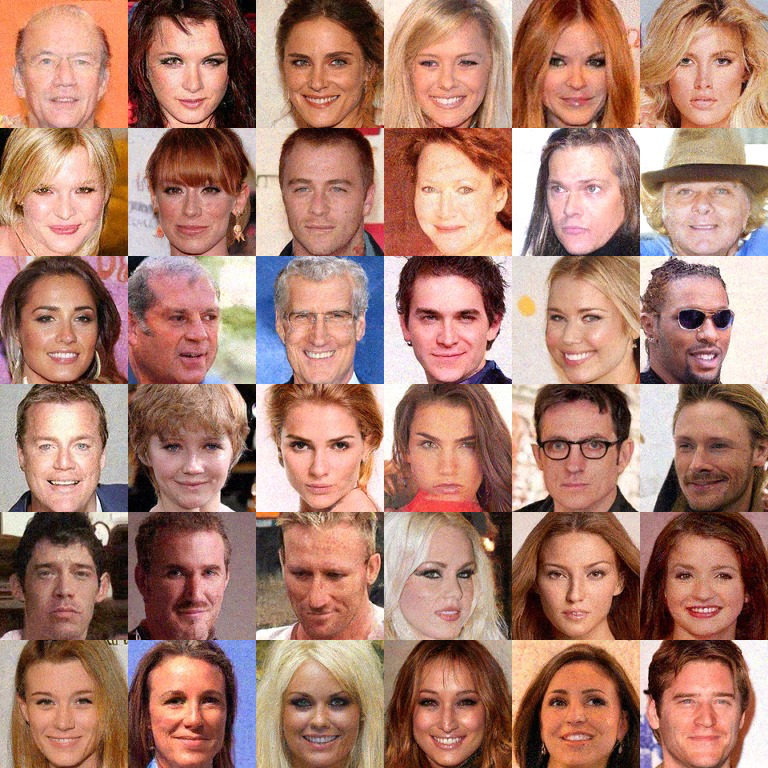
\includegraphics[width=\textwidth]{Chapter2/samples/multiscale/vanilla.png}
    \caption{Vanilla - CelebA-HQ $128\times 128$}
    \label{ch2:fig:Vanilla}
\end{figure*}

\begin{figure*}
    \centering
    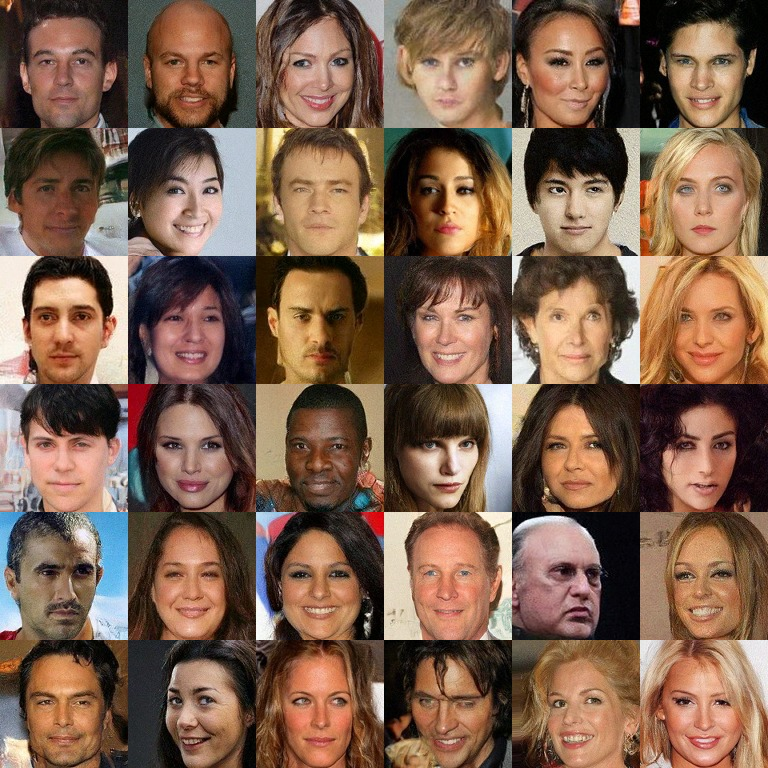
\includegraphics[width=\textwidth]{Chapter2/samples/multiscale/multiscale.png}
    \caption{Multiscale - CelebA-HQ $128\times 128$}
    \label{ch2:fig:Multiscale}
\end{figure*}

\begin{figure*}
    \centering
    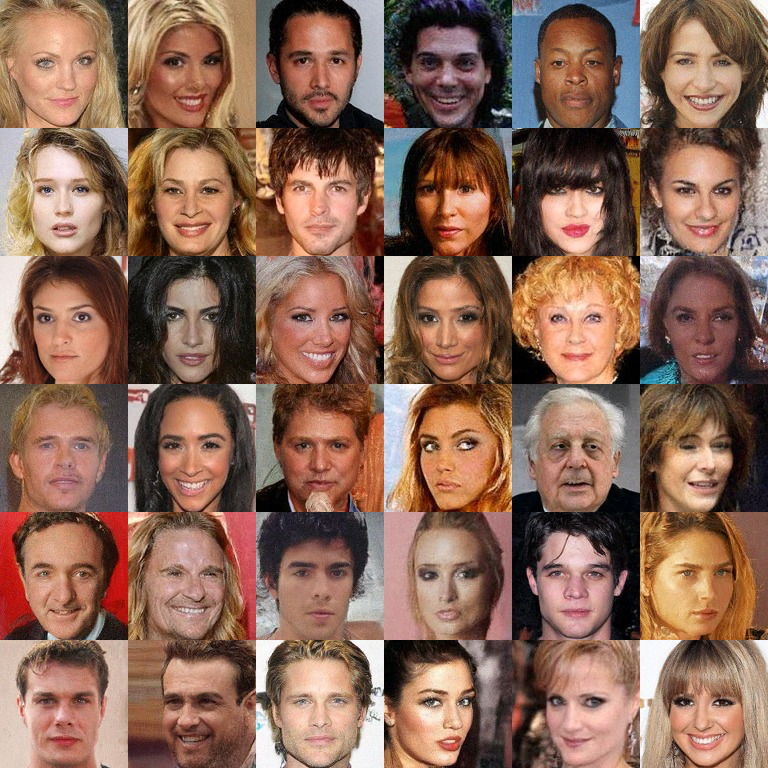
\includegraphics[width=\textwidth]{Chapter2/samples/multiscale/multiscale_deep.png}
    \caption{Multiscale + - CelebA-HQ $128\times 128$}
    \label{ch2:fig:Multiscale_+}
\end{figure*}



\begin{figure*}
    \begin{center}
    \begingroup
    \setlength{\tabcolsep}{0pt}
    %\renewcommand{\arraystretch}{1.5}
 
    \begin{tabular}{ccccccc}
        Original image $x$ & Observation $ y$ & HCFlow & CDE & CDiffE & CMDE & VS-CMDE \\

        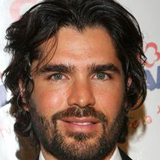
\includegraphics[width=.14\textwidth]{Chapter2/samples/extended_results/super_resolution/2/x.png} &   
        
\includegraphics[width=.14\textwidth]{Chapter2/samples/extended_results/super_resolution/2/y.png} &
        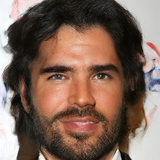
\includegraphics[width=.14\textwidth]{Chapter2/samples/extended_results/super_resolution/2/HCFLOW.png} &
        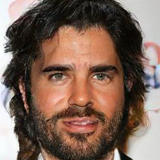
\includegraphics[width=.14\textwidth]{Chapter2/samples/extended_results/super_resolution/2/CDE.png} & 
        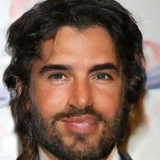
\includegraphics[width=.14\textwidth]{Chapter2/samples/extended_results/super_resolution/2/CDiffE.png} &
        \includegraphics[width=.14\textwidth]{Chapter2/samples/extended_results/super_resolution/2/cmde.png} &
        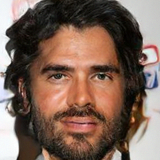
\includegraphics[width=.14\textwidth]{Chapter2/samples/extended_results/super_resolution/2/VS-CMDE.png}\\
        
        
\includegraphics[width=.14\textwidth]{Chapter2/samples/extended_results/super_resolution/8/x.png} &   
        
\includegraphics[width=.14\textwidth]{Chapter2/samples/extended_results/super_resolution/8/y.png} &
        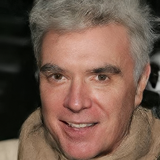
\includegraphics[width=.14\textwidth]{Chapter2/samples/extended_results/super_resolution/8/HCFLOW.png} &
        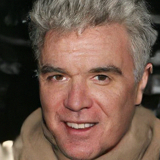
\includegraphics[width=.14\textwidth]{Chapter2/samples/extended_results/super_resolution/8/CDE.png} & 
        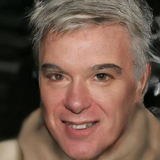
\includegraphics[width=.14\textwidth]{Chapter2/samples/extended_results/super_resolution/8/CDiffE.png} &
        \includegraphics[width=.14\textwidth]{Chapter2/samples/extended_results/super_resolution/8/cmde.png} &
        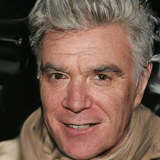
\includegraphics[width=.14\textwidth]{Chapter2/samples/extended_results/super_resolution/8/VS-CMDE.png}\\
        
        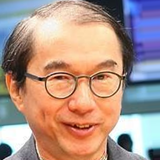
\includegraphics[width=.14\textwidth]{Chapter2/samples/extended_results/super_resolution/16/x.png} &   
        
\includegraphics[width=.14\textwidth]{Chapter2/samples/extended_results/super_resolution/16/y.png} &
        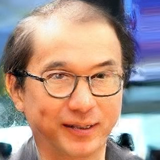
\includegraphics[width=.14\textwidth]{Chapter2/samples/extended_results/super_resolution/16/HCFLOW.png} &
        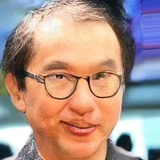
\includegraphics[width=.14\textwidth]{Chapter2/samples/extended_results/super_resolution/16/CDE.png} & 
        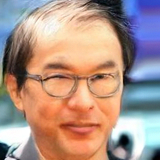
\includegraphics[width=.14\textwidth]{Chapter2/samples/extended_results/super_resolution/16/CDiffE.png} &
        \includegraphics[width=.14\textwidth]{Chapter2/samples/extended_results/super_resolution/16/cmde.png} &
        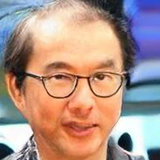
\includegraphics[width=.14\textwidth]{Chapter2/samples/extended_results/super_resolution/16/VS-CMDE.png}\\
        
        
\includegraphics[width=.14\textwidth]{Chapter2/samples/extended_results/super_resolution/59/x.png} &   
        
\includegraphics[width=.14\textwidth]{Chapter2/samples/extended_results/super_resolution/59/y.png} &
        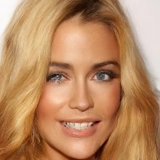
\includegraphics[width=.14\textwidth]{Chapter2/samples/extended_results/super_resolution/59/HCFLOW.png} &
        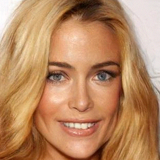
\includegraphics[width=.14\textwidth]{Chapter2/samples/extended_results/super_resolution/59/CDE.png} & 
        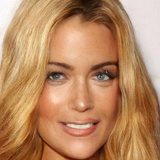
\includegraphics[width=.14\textwidth]{Chapter2/samples/extended_results/super_resolution/59/CDiffE.png} &
        \includegraphics[width=.14\textwidth]{Chapter2/samples/extended_results/super_resolution/59/cmde.png} &
        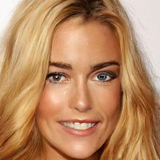
\includegraphics[width=.14\textwidth]{Chapter2/samples/extended_results/super_resolution/59/VS-CMDE.png}\\
        
        
\includegraphics[width=.14\textwidth]{Chapter2/samples/extended_results/super_resolution/111/x.png} &   
        
\includegraphics[width=.14\textwidth]{Chapter2/samples/extended_results/super_resolution/111/y.png} &
        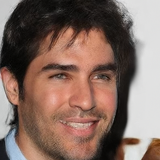
\includegraphics[width=.14\textwidth]{Chapter2/samples/extended_results/super_resolution/111/HCFLOW.png} &
        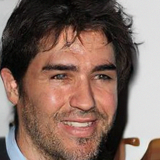
\includegraphics[width=.14\textwidth]{Chapter2/samples/extended_results/super_resolution/111/CDE.png} & 
        
\includegraphics[width=.14\textwidth]{Chapter2/samples/extended_results/super_resolution/111/CDiffE.png} &
        \includegraphics[width=.14\textwidth]{Chapter2/samples/extended_results/super_resolution/111/cmde.png} &
        
\includegraphics[width=.14\textwidth]{Chapter2/samples/extended_results/super_resolution/111/VS-CMDE.png}\\
        
        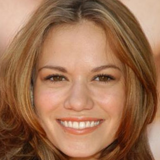
\includegraphics[width=.14\textwidth]{Chapter2/samples/extended_results/super_resolution/136/x.png} &   
        
\includegraphics[width=.14\textwidth]{Chapter2/samples/extended_results/super_resolution/136/y.png} &
        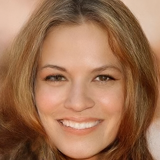
\includegraphics[width=.14\textwidth]{Chapter2/samples/extended_results/super_resolution/136/HCFLOW.png} &
        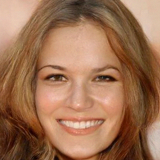
\includegraphics[width=.14\textwidth]{Chapter2/samples/extended_results/super_resolution/136/CDE.png} & 
        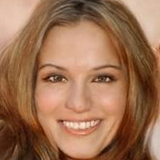
\includegraphics[width=.14\textwidth]{Chapter2/samples/extended_results/super_resolution/136/CDiffE.png} &
        \includegraphics[width=.14\textwidth]{Chapter2/samples/extended_results/super_resolution/136/cmde.png} &
        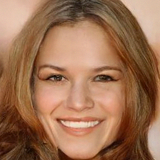
\includegraphics[width=.14\textwidth]{Chapter2/samples/extended_results/super_resolution/136/VS-CMDE.png}\\
        
        
\includegraphics[width=.14\textwidth]{Chapter2/samples/extended_results/super_resolution/164/x.png} &   
        
\includegraphics[width=.14\textwidth]{Chapter2/samples/extended_results/super_resolution/164/y.png} &
        
\includegraphics[width=.14\textwidth]{Chapter2/samples/extended_results/super_resolution/164/HCFLOW.png} &
        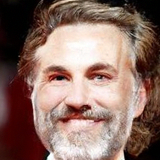
\includegraphics[width=.14\textwidth]{Chapter2/samples/extended_results/super_resolution/164/CDE.png} & 
        
\includegraphics[width=.14\textwidth]{Chapter2/samples/extended_results/super_resolution/164/CDiffE.png} &
        \includegraphics[width=.14\textwidth]{Chapter2/samples/extended_results/super_resolution/164/cmde.png} &
        \includegraphics[width=.14\textwidth]{Chapter2/samples/extended_results/super_resolution/164/VS-CMDE.png}\\
        
        \includegraphics[width=.14\textwidth]{Chapter2/samples/extended_results/super_resolution/805/x.png} &   
        \includegraphics[width=.14\textwidth]{Chapter2/samples/extended_results/super_resolution/805/y.png} &
        \includegraphics[width=.14\textwidth]{Chapter2/samples/extended_results/super_resolution/805/HCFLOW.png} &
        \includegraphics[width=.14\textwidth]{Chapter2/samples/extended_results/super_resolution/805/CDE.png} & 
        \includegraphics[width=.14\textwidth]{Chapter2/samples/extended_results/super_resolution/805/CDiffE.png} &
        \includegraphics[width=.14\textwidth]{Chapter2/samples/extended_results/super_resolution/805/cmde.png} &
        \includegraphics[width=.14\textwidth]{Chapter2/samples/extended_results/super_resolution/805/VS-CMDE.png}\\

    \end{tabular}
    \endgroup
    \end{center}
    \caption{Extended super-resolution results.}
    \label{ch2:fig:additional_sr}
\end{figure*}

\begin{figure*}
    \begin{center}
    \begingroup
    \setlength{\tabcolsep}{0pt}
    %\renewcommand{\arraystretch}{1.5}
 
    \begin{tabular}{ccccccc}
        Original image $x$ & Observation $ y$ & CDE & CDiffE & CMDE & VS-CMDE \\

        \includegraphics[width=.145\textwidth]{Chapter2/samples/extended_results/inpainting/7/x.png} &   
        \includegraphics[width=.145\textwidth]{Chapter2/samples/extended_results/inpainting/7/y.png} &
        \includegraphics[width=.145\textwidth]{Chapter2/samples/extended_results/inpainting/7/CDE.png} & 
        \includegraphics[width=.145\textwidth]{Chapter2/samples/extended_results/inpainting/7/CDiffE.png} &
        \includegraphics[width=.145\textwidth]{Chapter2/samples/extended_results/inpainting/7/cmde.png} &
        \includegraphics[width=.145\textwidth]{Chapter2/samples/extended_results/inpainting/7/VS-CMDE.png}\\
        
        \includegraphics[width=.145\textwidth]{Chapter2/samples/extended_results/inpainting/17/x.png} &   
        \includegraphics[width=.145\textwidth]{Chapter2/samples/extended_results/inpainting/17/y.png} &
        \includegraphics[width=.145\textwidth]{Chapter2/samples/extended_results/inpainting/17/CDE.png} & 
        \includegraphics[width=.145\textwidth]{Chapter2/samples/extended_results/inpainting/17/CDiffE.png} &
        \includegraphics[width=.145\textwidth]{Chapter2/samples/extended_results/inpainting/17/cmde.png} &
        \includegraphics[width=.145\textwidth]{Chapter2/samples/extended_results/inpainting/17/VS-CMDE.png}\\
        
        \includegraphics[width=.145\textwidth]{Chapter2/samples/extended_results/inpainting/20/x.png} &   
        \includegraphics[width=.145\textwidth]{Chapter2/samples/extended_results/inpainting/20/y.png} &
        \includegraphics[width=.145\textwidth]{Chapter2/samples/extended_results/inpainting/20/CDE.png} & 
        \includegraphics[width=.145\textwidth]{Chapter2/samples/extended_results/inpainting/20/CDiffE.png} &
        \includegraphics[width=.145\textwidth]{Chapter2/samples/extended_results/inpainting/20/cmde.png} &
        \includegraphics[width=.145\textwidth]{Chapter2/samples/extended_results/inpainting/20/VS-CMDE.png}\\
        
        \includegraphics[width=.145\textwidth]{Chapter2/samples/extended_results/inpainting/21/x.png} &   
        \includegraphics[width=.145\textwidth]{Chapter2/samples/extended_results/inpainting/21/y.png} &
        \includegraphics[width=.145\textwidth]{Chapter2/samples/extended_results/inpainting/21/CDE.png} & 
        \includegraphics[width=.145\textwidth]{Chapter2/samples/extended_results/inpainting/21/CDiffE.png} &
        \includegraphics[width=.145\textwidth]{Chapter2/samples/extended_results/inpainting/21/cmde.png} &
        \includegraphics[width=.145\textwidth]{Chapter2/samples/extended_results/inpainting/21/VS-CMDE.png}\\
        
        \includegraphics[width=.145\textwidth]{Chapter2/samples/extended_results/inpainting/47/x.png} &   
        \includegraphics[width=.145\textwidth]{Chapter2/samples/extended_results/inpainting/47/y.png} &
        \includegraphics[width=.145\textwidth]{Chapter2/samples/extended_results/inpainting/47/CDE.png} & 
        \includegraphics[width=.145\textwidth]{Chapter2/samples/extended_results/inpainting/47/CDiffE.png} &
        \includegraphics[width=.145\textwidth]{Chapter2/samples/extended_results/inpainting/47/cmde.png} &
        \includegraphics[width=.145\textwidth]{Chapter2/samples/extended_results/inpainting/47/VS-CMDE.png}\\
        
        \includegraphics[width=.145\textwidth]{Chapter2/samples/extended_results/inpainting/68/x.png} &   
        \includegraphics[width=.145\textwidth]{Chapter2/samples/extended_results/inpainting/68/y.png} &
        \includegraphics[width=.145\textwidth]{Chapter2/samples/extended_results/inpainting/68/CDE.png} & 
        \includegraphics[width=.145\textwidth]{Chapter2/samples/extended_results/inpainting/68/CDiffE.png} &
        \includegraphics[width=.145\textwidth]{Chapter2/samples/extended_results/inpainting/68/cmde.png} &
        \includegraphics[width=.145\textwidth]{Chapter2/samples/extended_results/inpainting/68/VS-CMDE.png}\\
        
        \includegraphics[width=.145\textwidth]{Chapter2/samples/extended_results/inpainting/111/x.png} &   
        \includegraphics[width=.145\textwidth]{Chapter2/samples/extended_results/inpainting/111/y.png} &
        \includegraphics[width=.145\textwidth]{Chapter2/samples/extended_results/inpainting/111/CDE.png} & 
        \includegraphics[width=.145\textwidth]{Chapter2/samples/extended_results/inpainting/111/CDiffE.png} &
        \includegraphics[width=.145\textwidth]{Chapter2/samples/extended_results/inpainting/111/cmde.png} &
        \includegraphics[width=.145\textwidth]{Chapter2/samples/extended_results/inpainting/111/VS-CMDE.png}\\
        
        \includegraphics[width=.145\textwidth]{Chapter2/samples/extended_results/inpainting/146/x.png} &   
        \includegraphics[width=.145\textwidth]{Chapter2/samples/extended_results/inpainting/146/y.png} &
        \includegraphics[width=.145\textwidth]{Chapter2/samples/extended_results/inpainting/146/CDE.png} & 
        \includegraphics[width=.145\textwidth]{Chapter2/samples/extended_results/inpainting/146/CDiffE.png} &
        \includegraphics[width=.145\textwidth]{Chapter2/samples/extended_results/inpainting/146/cmde.png} &
        \includegraphics[width=.145\textwidth]{Chapter2/samples/extended_results/inpainting/146/VS-CMDE.png}\\
        
        
    \end{tabular}
    \endgroup
    \end{center}
    \caption{Extended inpainting results.}
    \label{ch2:fig:additional_inpainting}
\end{figure*}

\begin{figure*}
    \begin{center}
    \begingroup
    \setlength{\tabcolsep}{2.5pt}
    \begin{tabular}{lcccccccc}
        \begin{tabular}{@{}l@{}}
            Original image $x$
            \\[25pt]
        \end{tabular}
         & \includegraphics[width=.08\textwidth]{Chapter2/samples/extended_results/edges-to-shoes/1/x.png} & \includegraphics[width=.08\textwidth]{Chapter2/samples/extended_results/edges-to-shoes/6/x.png} & \includegraphics[width=.08\textwidth]{Chapter2/samples/extended_results/edges-to-shoes/8/x.png} &
         \includegraphics[width=.08\textwidth]{Chapter2/samples/extended_results/edges-to-shoes/10/x.png} &
         \includegraphics[width=.08\textwidth]{Chapter2/samples/extended_results/edges-to-shoes/21/x.png} &
         \includegraphics[width=.08\textwidth]{Chapter2/samples/extended_results/edges-to-shoes/99/x.png} &
         \includegraphics[width=.08\textwidth]{Chapter2/samples/extended_results/edges-to-shoes/126/x.png} &
         \includegraphics[width=.08\textwidth]{Chapter2/samples/extended_results/edges-to-shoes/134/x.png} \\
        
        \begin{tabular}{@{}l@{}}
            Observation \\ $ y := Ax$
            \\[25pt]
        \end{tabular}
         & \includegraphics[width=.08\textwidth]{Chapter2/samples/extended_results/edges-to-shoes/1/y.png} & \includegraphics[width=.08\textwidth]{Chapter2/samples/extended_results/edges-to-shoes/6/y.png} & \includegraphics[width=.08\textwidth]{Chapter2/samples/extended_results/edges-to-shoes/8/y.png} &
         \includegraphics[width=.08\textwidth]{Chapter2/samples/extended_results/edges-to-shoes/10/y.png} &
         \includegraphics[width=.08\textwidth]{Chapter2/samples/extended_results/edges-to-shoes/21/y.png} &
         \includegraphics[width=.08\textwidth]{Chapter2/samples/extended_results/edges-to-shoes/99/y.png} &
         \includegraphics[width=.08\textwidth]{Chapter2/samples/extended_results/edges-to-shoes/126/y.png} &
         \includegraphics[width=.08\textwidth]{Chapter2/samples/extended_results/edges-to-shoes/134/y.png} \\
        
         \begin{tabular}{@{}c@{}}
            CDE
            \\[25pt]
        \end{tabular} & 
            \includegraphics[width=.08\textwidth]{Chapter2/samples/extended_results/edges-to-shoes/1/CDE.png} & \includegraphics[width=.08\textwidth]{Chapter2/samples/extended_results/edges-to-shoes/6/CDE.png} & \includegraphics[width=.08\textwidth]{Chapter2/samples/extended_results/edges-to-shoes/8/CDE.png} &
            \includegraphics[width=.08\textwidth]{Chapter2/samples/extended_results/edges-to-shoes/10/CDE.png} &
            \includegraphics[width=.08\textwidth]{Chapter2/samples/extended_results/edges-to-shoes/21/CDE.png} &
            \includegraphics[width=.08\textwidth]{Chapter2/samples/extended_results/edges-to-shoes/99/CDE.png} &
            \includegraphics[width=.08\textwidth]{Chapter2/samples/extended_results/edges-to-shoes/126/CDE.png} &
            \includegraphics[width=.08\textwidth]{Chapter2/samples/extended_results/edges-to-shoes/134/CDE.png} \\

        \begin{tabular}{@{}c@{}}
            CMDE (Ours)
            \\[25pt]
        \end{tabular}  &  
            \includegraphics[width=.08\textwidth]{Chapter2/samples/extended_results/edges-to-shoes/1/CMDE.png} & \includegraphics[width=.08\textwidth]{Chapter2/samples/extended_results/edges-to-shoes/6/CMDE.png} & \includegraphics[width=.08\textwidth]{Chapter2/samples/extended_results/edges-to-shoes/8/CMDE.png} &
            \includegraphics[width=.08\textwidth]{Chapter2/samples/extended_results/edges-to-shoes/10/CMDE.png} &
            \includegraphics[width=.08\textwidth]{Chapter2/samples/extended_results/edges-to-shoes/21/CMDE.png} &
            \includegraphics[width=.08\textwidth]{Chapter2/samples/extended_results/edges-to-shoes/99/CMDE.png} &
            \includegraphics[width=.08\textwidth]{Chapter2/samples/extended_results/edges-to-shoes/126/CMDE.png} &
            \includegraphics[width=.08\textwidth]{Chapter2/samples/extended_results/edges-to-shoes/134/CMDE.png} \\
    \end{tabular}
    \endgroup
    \end{center}
    \caption{Extended edge to shoe synthesis results.}
    \label{ch2:fig:additional_shoe}
\end{figure*}

\section{Potential negative impact}
The potential of negative impact of this work is the same as that of any work that advances generative modelling. Generative modelling can be used for the creation of deep-fakes which can be used for malicious purposes such as disinformation and blackmailing. However, research on generative modelling can indirectly or directly contribute to the robustification of deep-fake detection algorithms. Moreover, generative models have proven very useful in academic research and in industry. The potential benefits of generative modelling outweigh the potential threats. Therefore, the research community should continue to conduct research on generative modelling.